%%%%%%%%%%%%%%%%%%%%%%%%%%%%%%%%%%%%%%%%%%%%%%%%%%%%%%%%%%%%%%%%%%%%%%%%%%%%%%%%%%%%%%
% This LaTeX file was prepared by:
%       Debdeep Mukhopadhyay and Abhishek Somani
%       Associate Professor and Principal Engineer
%       Dept. of Computer Science and Engineering
%       IIT Kharagpur
%       Kharagpur, India - 721302
%       Mentor Graphics, India
%       E-mail: debdeep@cse.iitkgp.ernet.in, abhishek.somani@gmail.com 
%       Last Modified: 2nd August, 2015
%%%%%%%%%%%%%%%%%%%%%%%%%%%%%%%%%%%%%%%%%%%%%%%%%%%%%%%%%%%%%%%%%%%%%%%%%%%%%%%%%%%%%%
\documentclass{article}
\usepackage[pdftex]{color,graphicx}
\usepackage{amsmath}
\usepackage{amssymb}
%\usepackage{pdfpages}
%\usepackage{listings}
%\usepackage{algorithm}
%\usepackage{algpseudocode}
%\usepackage{algorithmic}
\usepackage{enumerate}
\usepackage{syntonly}
\usepackage{multicol}
\usepackage{array}
\usepackage{mathrsfs}  
%\usepackage[tight,footnotesize]{subfigure}
%\usepackage{stfloats}
%\usepackage{url}
%\usepackage{threeparttable}
%\usepackage{cite}
\usepackage{exam}

%\usepackage{algorithmic}

\usepackage{algorithm}
\usepackage{algcompatible}

\algblockdefx{FORALLP}{ENDFAP}[1]%
  {\textbf{for all }#1 \textbf{do in parallel}}%
  {\textbf{end for}}

\paper{CS60004}  % <- do not include FC, FT etc
%\version{0}                     % <- for multiple choice exams
\subject{CS60004: Hardware Security}
\title{Mid-Term Examination}
\time{2}                      % <- number of hours: default is three
\semester{Spring}
\year{2018}                     % <- default is the current year
%\campus{Shanghai}
\fullmarks{40}
\note{Attempt all Questions. \newline
}

\begin{document}

\begin{questions}

\question 

\begin{enumerate}
 \item Consider the following $4$-input boolean function:
\begin{equation}
 f\left(x_1,x_2,x_3,x_4\right) = \left(x_1 \cdot x_2\right) + \left(x_3 \cdot x_4\right)\nonumber
\end{equation}
\noindent Describe a gate-level masked implementation of this boolean function.\marks{7}
\end{enumerate}





\question 

Consider a substitution-permutation network with a $64$-bit state and a $64$-bit round key described in Figure~\ref{fig:present_structure}, where $\mathrm{\mathbf{S}}$ is a non-linear $4\times 4$ S-Box. Observe that the S-Box layer is followed by a bit-permutation layer and a bit-wise round-key XOR layer. Note that a \emph{nibble} is a collection of 4 consecutive bits (a 4-bit equivalent of a byte). Also, assume that the expected number of solutions to the equation:
\begin{equation}
 \mathrm{\mathbf{S}}^{-1}\left(x\right) \oplus \mathrm{\mathbf{S}}^{-1}\left(x\oplus A\right) = B\nonumber
\end{equation}
\noindent for known $A$ and $B$ and unknown $x$ is $1$.

\begin{figure}[h]
	\centering
	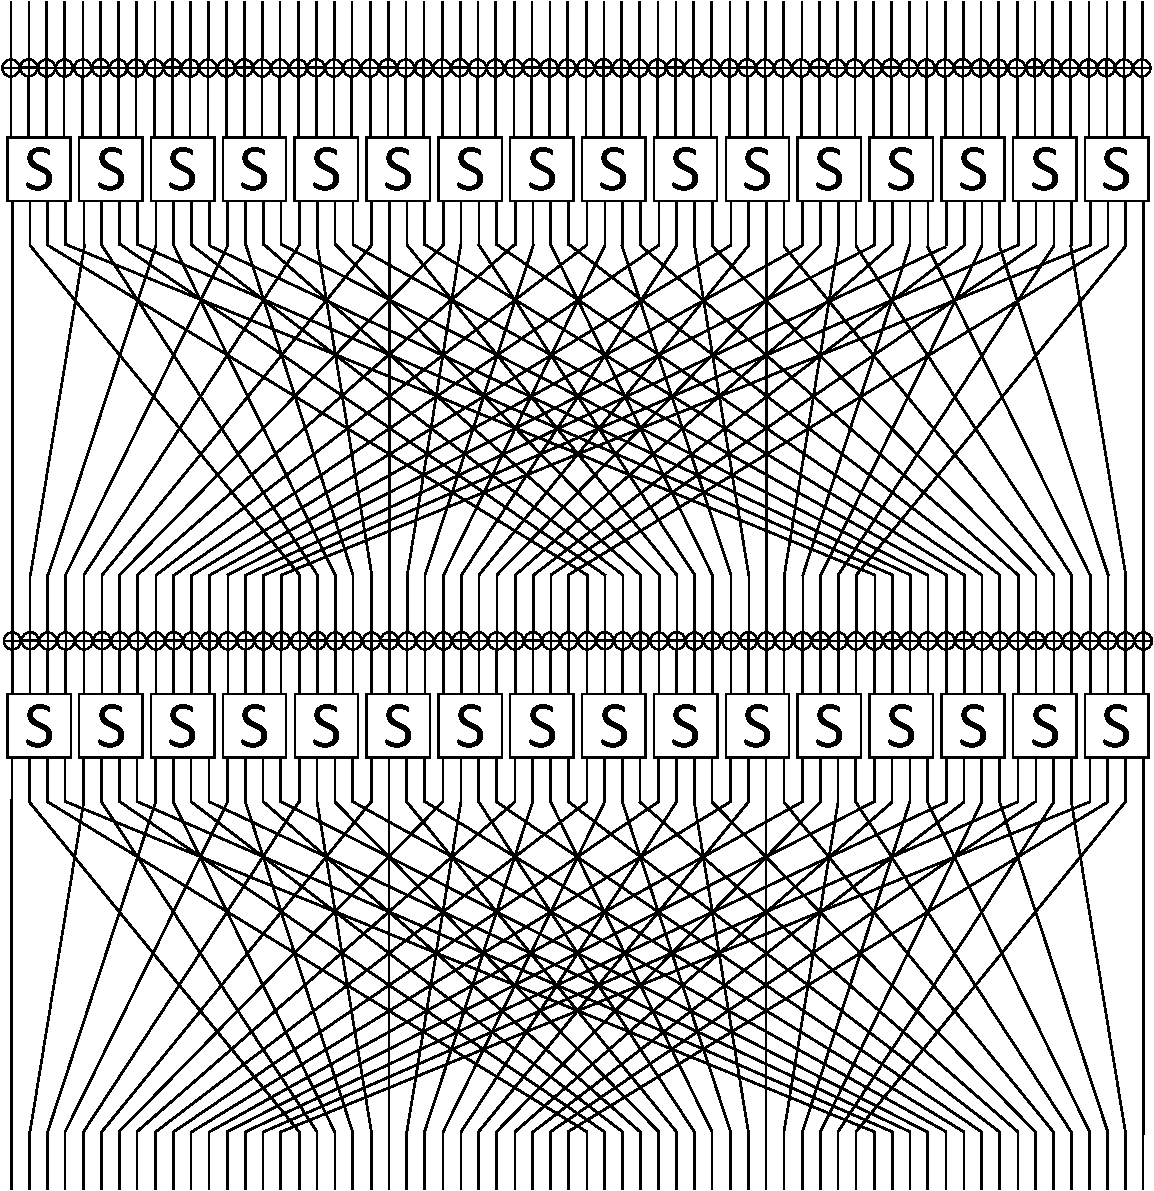
\includegraphics[scale=0.3]{present_structure.pdf}
    \caption{To rounds of a substitution-permutation network}
    \label{fig:present_structure}
\end{figure}


\begin{enumerate}
 \item Suppose an attacker introduces a \emph{fixed} single-nibble fault of Hamming Weight $x$ at the input of round $r$ in an iterated implementation of this SPN structure. Prove that the faulty input value for any nibble in round $\left(r+2\right)$ takes at most $2^x$ values.\marks{7}
 
 \item Now consider a practical fault attack in which an adversary can actually inject a specific (and known) single-nibble fault of Hamming Weight $x$ at the input of round $r$ in an iterated implementation of this SPN structure Weight $x$. Describe a fault attack methodology to recover the $\left(r+2\right)^{\textnormal{th}}$ round-key from the correct and faulty outputs of the $\left(r+2\right)^{\textnormal{th}}$ round of this SPN structure. \marks{6}
 
 \item Remark on the possible values of $x$ for which the fault attack is practically feasible, and the expected number of fault injections required for each such $x$ for complete key-recovery \marks{2} 
 
\end{enumerate}







\end{questions}
\end{document}
